\section{Introduction to vivado HLS}
This first task was an introduction in Vivado and Vivado HLS. The tutorial provided sample code of an FIR (Finite Impulse response) filter. One of the main focuses of lab 1 was to convert the high-level C code into RTL implementation, so that it could be used later for the Vivado application. Vivado HLS provides a Graphical User Interface, making the design flow more clear to follow and debug. 
 
The next main part of that tutorial was the validation of the C code. A process called C Simulation checks if the written C Code works correctly by comparing its output data to some predefined right result. The comparison is being done in a separate test bench which is also written in C. The test bench contains a function that compiles the written C code, compares its output to the predefined result and returns a 0 or 1 if the outputs matched or not. Once the C code is checked, it can be used in a C Synthesis.
The next step was to perform the High-level synthesis. C Synthesis generates an Register Transfer Level (RTL) design for the written C code and reports on its estimated performance. The report includes a utilization estimate, showing an approximate number of flip-flops (FF), look-up tables (LUT), digital signal processors (DSPs) and block ram (BRAM) needed in the design. A precise number cannot be evaluated prior to the RTL synthesis since there could be additional optimizations.

The next step was the RTL verification. Just like the C code, the RTL design has to be tested in an RTL co-simulation (source RTL explanation). The C test bench can be reused.\cite[p.25]{xilinx2018}
The last step was the IP creation of the design. In order to use the RTL design it has to be exported from Vivado HLS as an IP block 

The purpose of Lab 3 was to understand different solutions to optimize an HLS design. The main goal here was to process and output binary data with the highest possible throughput.
The first performed optimization was on the I/O interfaces, predefining how the design can be optimized later on. The C Synthesis showed that the “Shift\_Accum\_Loop” was unrolled completely in order to increase performance. Unrolling the loop increases: throughput, time taken for the system to be ready to receive the next input, and latency, which is the time taken for the system to give an output.

Another point was that since “y” is an input port, it is important to store the result in a separate variable “acc” before passing it to “y”, which PYNQ’s PL system is perfectly made for with DSPs for high-speed arithmetic.\cite[p.25]{crockettelliottenderwitzstewart2014}\\

\section{Introduction into PYNQ and Overlay Design}
In the next task, the group has changed the variables’ data types to smaller bit sizes. This resulted in fewer clock cycles and reduced hardware. As shown below, the amount of Look-Up Tables and FlipFlops has been reduced to about a third and the latency to about 80\%.


\begin{figure}[h]
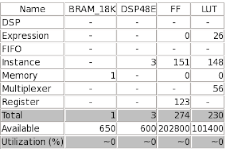
\includegraphics[scale=1.2]{lefttable}
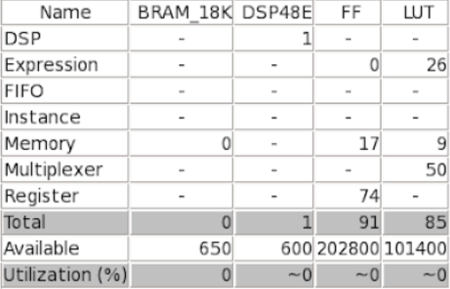
\includegraphics[scale=0.62]{righttable}
\caption{Results before on the left, results after on the right.}
\label{resulttable}
\end{figure}

Next, the test-bench was modified to calculate the RMSE between the software and simulated custom precision hardware implementation. This is useful in terms of understanding how accurate the implementation can be. (Code is in Appendix A.1)

\begin{figure}[h]
\centering
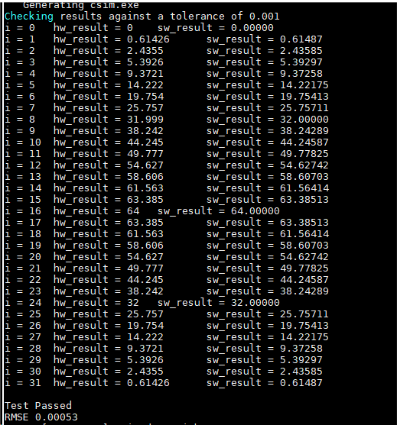
\includegraphics[scale=1]{RMSE}
\caption{Output of the simulation with RMSE code}
\label{RMSE}
\end{figure}




\section{ Design of a dot-product module}
The group were next tasked in designing a hardware module in Vivado HLS, which calculates the dot-product of two vectors. The module takes as input the two vectors in an array form and outputs the dot-product as an integer. This function is called upon by the test bench (displayed in the appendix), and compares the output with the expected answer calculated by the software. When the group tested this, an unroll factor was used to optimise the hardware. “Unrolling” the code is a term describing the process of repeating the blocks required for this function to reduce the number of iterations or “trips” of the loop required. \cite[p.321]{crockettelliottenderwitzstewart2014} Therefore, instead of using the same hardware over and over, the code can send data concurrently to the hardware, in turn reducing the latency of the system and increasing the throughput. Looking at the table below, an observation can be made showing that increasing the unroll factor causes more use of hardware, but decreases the throughput. In this task, the group chose the array size to be 10, so the loop had to run only 10 times, therefore an unroll factor of 10 has fully unrolled the loop making the most of the pipelining and also making the hardware more complex. An unroll factor higher than that for this task would make no difference, as the loop is fully unrolled.


\begin{figure}[h]
\centering
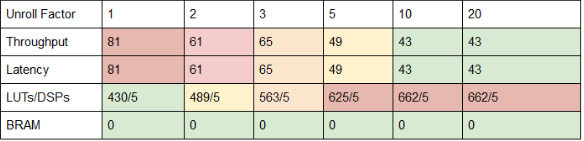
\includegraphics[scale=1]{unrolltable}
\caption{Comparison of effect of different unroll factors}
\label{unrolltable}
\end{figure}


\section{Creating a program to interact with Overlay on the PYNQ board.}

In the next task, the team was introduced to the actual PYNQ board. The group were given instructions on how to connect and set up the PYNQ board and use the Jupiter environment to compile and upload python to the CPU. Jupiter’s Edit and Command mode allow testing of  individual cells, making organizing and debugging much more efficient. The python software scripts written in the Jupyter Notebook interact with PYNQ’s programmable logic (PL) by running on its processing system (PS) via the AXI interface.\cite[p.6]{crockettelliottenderwitzstewart2014}

The task was to create a binary counter (code in the Appendix A.4). For debugging purposes the team made some code for service LEDs to flash when the code is uploaded. The team has also decreased the timing between each individual count.


\section{Overlay design}

The next task on the PYNQ board that the team tackled was to create a number adding program (See the appendix for code). Once again, a Vivado HLS with the “NumAdd” C code and needed directives was created. All inputs and outputs have been set to Slave lite interface so that they could communicate with the CPU\cite[p.299]{crockettelliottenderwitzstewart2014}. Running the synthesis to convert into HDL showed that the addition was implemented using LUTs instead of DSPs. 

The next step was to add an HDL wrapper to the design and generate the bitstream, allowing it to be used for the PL on the PYNQ board. In the end, the team has generated the .tcl file, containing the project block diagram. PYNQ board uses the tcl script to identify the configuration system and IP data such as control signals, for interface with the PS.
The final step was to record the address data for the overlay ports so that the PS would know how to reference the read/write ports of the block. The address attributed to the block was at the offset of 0x43C0\_0000 with the highest address of 0x43C0\_FFFF and range of 64k. Then, the team also recorded the address of the inputs and outputs inside the block, which were 0x00 for the control signals, 0x10 for signal a, 0x18 for signal b and 0x20 for signal y.  The data signals were predefined in the C code as 32-bit data ports.

In the final step, the custom overlay, which is used for file creation on the PYNQ FPGA and MMIO were loaded onto the PYNQ board and interfaced via different classes. 

To manage the communication with the PL, the group has used control signals such as ap\_start. This triggers blocks calculation and ap\_done, which in turn allows the team to get feedback when the results are ready to be read. There are other control signals that could be used such as ap\_ready (when the block is ready for the new input) and ap\_idle, which indicates if the block is operating or currently idle\cite[p.303]{crockettelliottenderwitzstewart2014}. The code has been adjusted to allow the calculation to take more than one cycle, via the use of ap\_done, before reading the output.


\section{Starting with PYNQ Video Processing and Computer Vision Reference Design.}

The team started with sending the HDMI signal through the PYNQ board the team got 60FPS. However, when turned on grayscaling the FPS dropped significantly to below 10FPS, which was expected, but not to this extent.

The next step was to move onto edge detection algorithms, as the tutorial sheet suggests. The given code imports an image and performs edge detection on it and saves it as a new file (See Figure \ref{edgedetection}). The C Synthesis estimated the following hardware usage (See table \ref{ResourceUse}). Since the dimensions of the image are undefined at execution time, there is no latency prediction in the synthesis. By redefining the image size, the number of loop executions and hence the timing can be estimated. The team synthesised the hardware block design in Vivado. Shown below are the hardware resources needed in the actual design. There is a noticeable increase in resource usage, due to the fact that Vivado HLS only gives value for the block designed, while Vivado adds all the interface and integration blocks in order for the PL and PS to function together. 

\begin{figure}[h]
    \centering
    \begin{subfigure}[b]{0.6\textwidth}
        \centering
        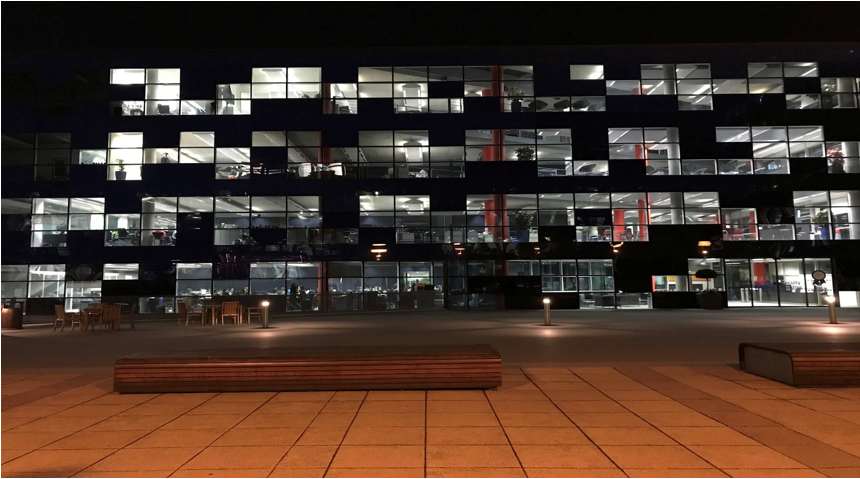
\includegraphics[width=\textwidth]{beforefilter}
        \caption{Initial image}
        \label{beforefilter}
    \end{subfigure}
    \begin{subfigure}[b]{0.6\textwidth}
        \centering
        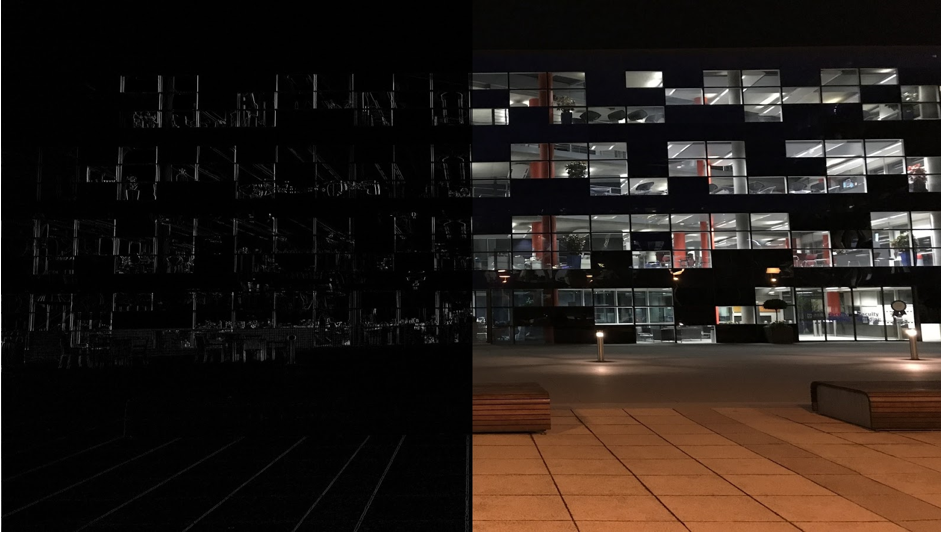
\includegraphics[width=\textwidth]{afterfilter}
        \caption{Half the image edge detected}
        \label{afterfilter}
    \end{subfigure}
    \hfill
    \caption{Demonstration of edge detection on half the image}
    \label{edgedetection}
\end{figure}


\begin{table}[h]
\centering
\begin{tabular}{ |p{3cm}||p{2cm}|p{2cm}|p{2cm}|p{2cm}|}
 \hline
 SOFTWARE & BRAM\_18K & DSP48E & FF & LUT\\
 \hline
 \hline
 Vivado HLS   & 2 & 13 &  3841 & 5809\\
 Vivado & 64 & 31 & 61462 & 40028 \\
 \hline
\end{tabular}
\caption{Comparison of resource use between Vivado HLS and Vivado.}
\label{ResourceUse}
\end{table}

\section{Modifying the design to add Horizontal Edge detection.}

The final step was to implement horizontal edge detection. If one would just rewrite the vertical edge detection code, changing the horizontal and vertical variables, the design would be extremely inefficient since the “in\_data” pointer would have to jump around in the memory. This is the case since the data of the image is stored in such a way, that once the pointer is incremented it points to the next pixel on the x-axis, but not on the y-axis. Hence, the group decided to use a buffer that stores the grey values of the whole previous row, for which they used an array with the image width as its predefined size (and further predefined the image width and height). Calculating the difference between each “grayscale pixel” from the current and the last row thus avoids the jumping (see code in the appendix A.5). For output of the program see Figure \ref{horizontaledge}.


\begin{figure}[H]
\centering
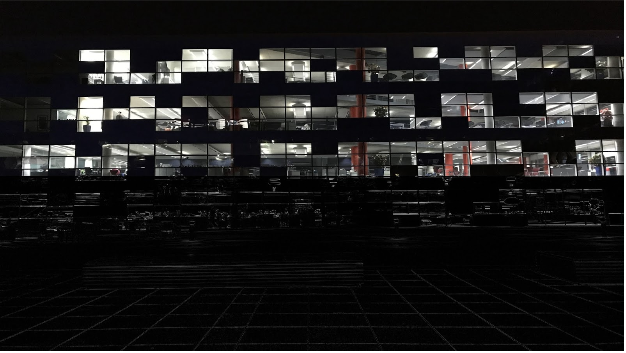
\includegraphics[scale=0.8]{horizontaledge}
\caption{Horizontal edge filter output}
\label{horizontaledge}
\end{figure}

Both the vertical and horizontal edge detection algorithms require approximately the same amount of hardware apart from BRAM (see Table \ref{ResourceUseEdge}). This can be traced back to the extra array the horizontally operating algorithm uses.

\begin{table}[H]
\centering
\begin{tabular}{ |p{3cm}||p{2cm}|p{2cm}|p{2cm}|p{2cm}|}
 \hline
 SOFTWARE & BRAM\_18K & DSP48E & FF & LUT\\
 \hline
 \hline
 Vertical   & 2 & 13 &  3841 & 5809\\
 Horizontal & 6 & 13 & 4248 & 5795 \\
 \hline
\end{tabular}
\caption{Comparison of resource use between Vertical and Horizontal edge detection filters.}
\label{ResourceUseEdge}
\end{table}





